\section{Knowledge model}


\subsection{Domain knowledge}
In our context analysis we identified four different kinds of knowledge shown in tables TM-2. This knowledge is all domain knowledge but they are represented in different ways in out model. The general car knowledge would be a car template, a concept that is part of our domain schema. Because we did not implement the ability for our system to reason with car templates we do not have an instantiation of such a template.

A simplified instantiation of specific car knowledge is shown in figures~\ref{fig:ChargeSystem},~\ref{fig:LightSystem} and~\ref{fig:StartAndIgnitionSystem}. These figures show exactly which components exist and how they are connected in our example car. A part of this knowledge is also present in our knowledge base since the components since the mappings between component states and observables can be different for every car. There exist many different cars and every car would have its own scheme. Modeling them is beyond the scope of this project.

Component knowledge is contained in our knowledge base. These are the rules that state exactly what happens when two components are connected. Note that these rules do not specify specific components and they are thus independent of the actual car.

Car repair knowledge is not present in our model. This is because our system does not use car repair knowledge for reasoning. Adding car repair knowledge could enhance the system by enabling it to propose observables that are easy to observe first.

\subsubsection{Domain schema}
The domain schema shown in figure~\ref{fig:DS} shows that a car `consists of' electrical parts and that these parts can be of several types. Connections are special because they are electrical components that connect other components. The rule types shown in figure~\ref{fig:IS} define the rules that exist between these concepts. 

\begin{figure}[htbp]
	\centering
		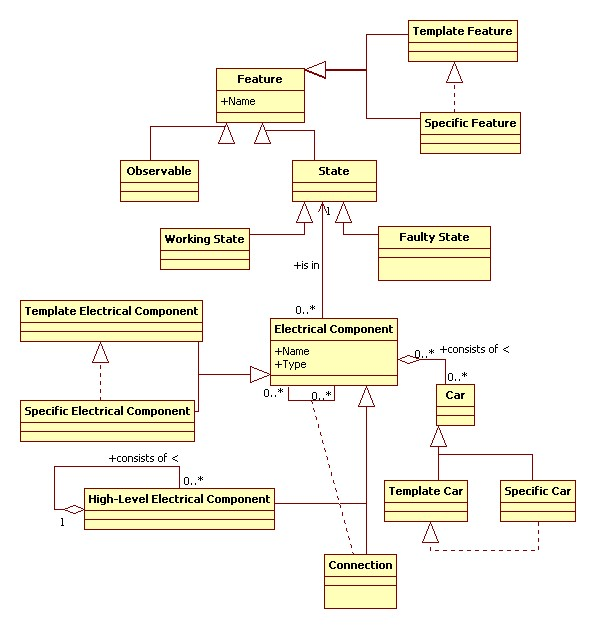
\includegraphics[width=1.00\textwidth]{DomainSchema.jpg}
	\caption{Domain schema for the car diagnoses task}
	\label{fig:DS}
\end{figure}

\begin{figure}[htbp]
	\centering
	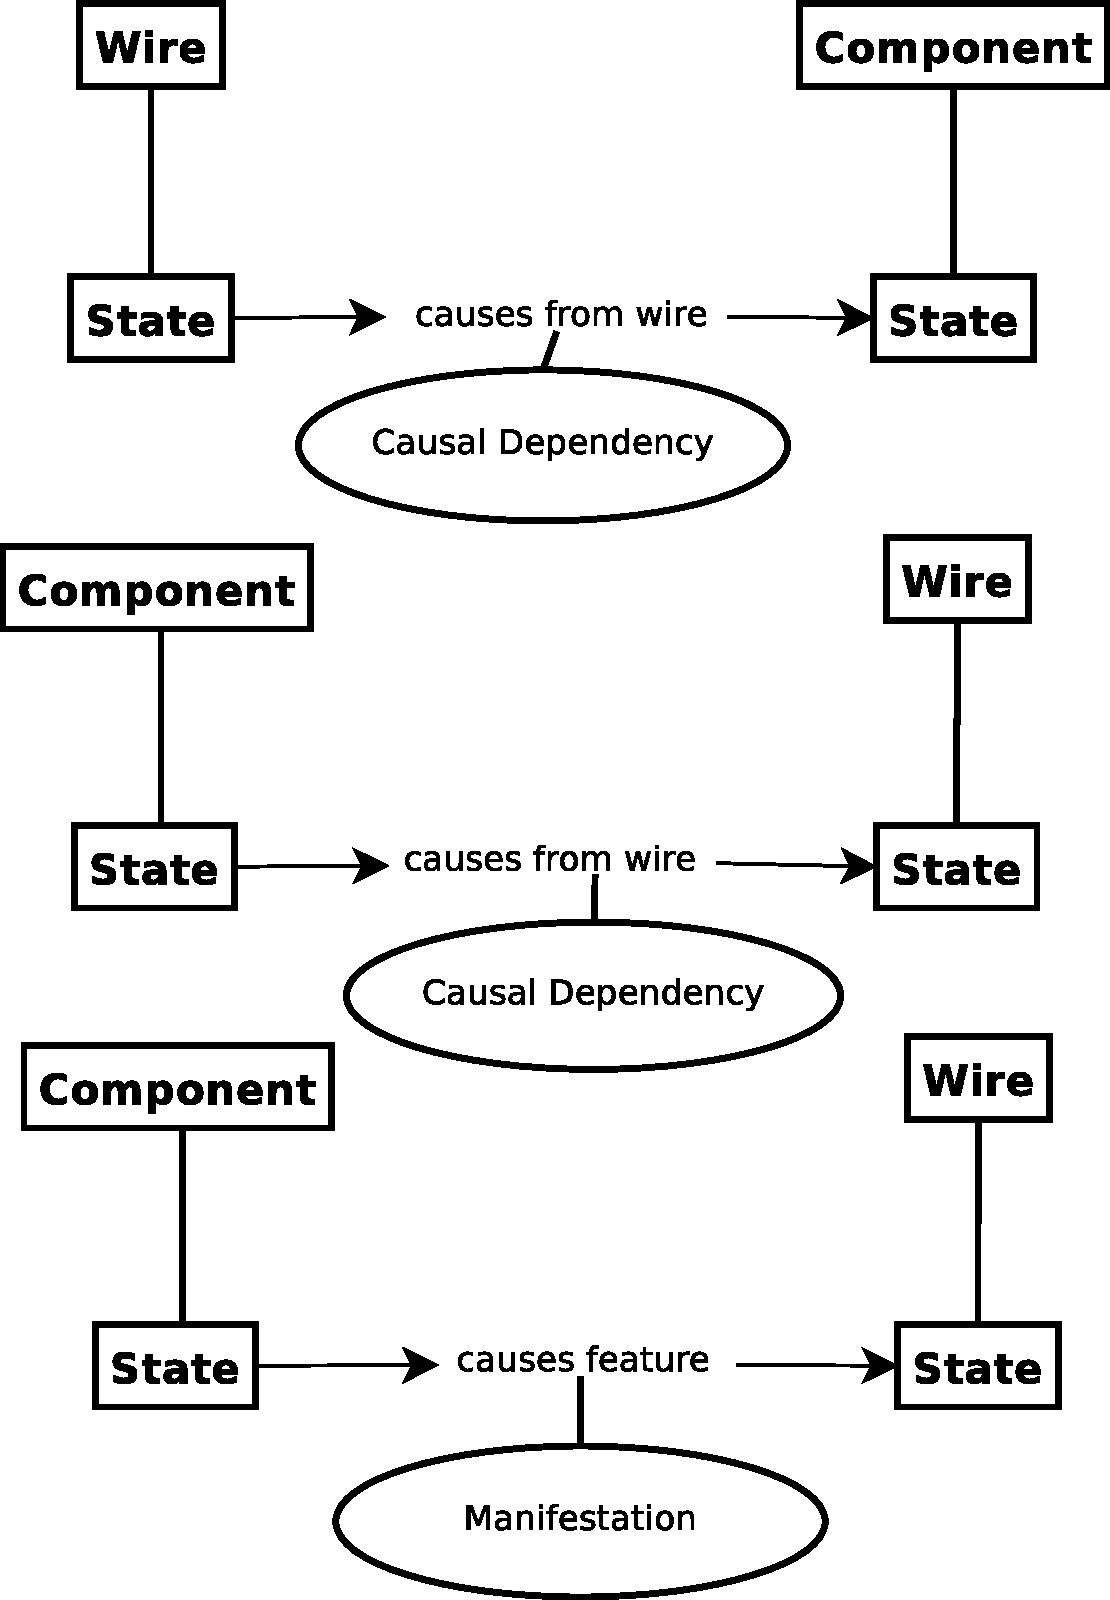
\includegraphics[width=7cm]{rule-types.pdf}
	\caption{Rule types}
	\label{fig:IS}
\end{figure}

\subsubsection{Knowledge base}
Below is a general overview of our knowledge base. Because all rules together create a single causal model all rules are contained in a single knowledge base. Not all rules are shown. Instead we show one instance of every kind of rule and explain how the other rules look. This is done because the complete knowledge base is very large.

The CAUSES-TO-WIRE rules state that if a device is generating or passing through power and this device is in a state that makes it unable to perform this function then all wires leading from it will not be powered. A separate rule exists for the combinations of each device type with every possible state that would make it unable to power the wire.

\begin{verbatim}
KNOWLEDGE-BASE causal-model;
   USES:
      Component-knowledge
      Car-specific-knowledge
   EXPRESSIONS:
      A.state = empty
      A.type = battery
      B.type = connection
      B.comp1 = A
      CAUSES-TO-WIRE
      B.state = no-power
\end{verbatim}

\noindent
The CAUSES-FROM-WIRE rules state that if all wires connected to a device are in a state that makes them unable to pass on power then this device will not be powered. A separate rule exists for the combination of every wire state that makes the wire unable to pass on power and every device type.

\begin{verbatim}
      A.state = empty
      A.type = battery
      B.type = connection
      B.comp1 = A
      CAUSES-FROM-WIRE
      B.state = no-power
\end{verbatim}

\noindent
The CAUSES-FEATURE rules map states of actual devices to observables. A separate rule exists for the combination of every device with all of its possible states that cause an observable. Note that these rules are not general and are dependend on the car. Thus these rules represent specific car knowledge.

\begin{verbatim}
      A.name = head-light-left
      A.state = no-power
      CAUSES-FEATURE
      observable = head-light-left-no-light
END KNOWLEDGE-BASE causal-model;
\end{verbatim}


\subsubsection{Example of a car}
Figures~\ref{fig:ChargeSystem},~\ref{fig:LightSystem} and~\ref{fig:StartAndIgnitionSystem} show a graphical representation of an example car according to our model. This car consists of several electrical components. Normal electrical components are shown as objects in boxes with underlined text. Connections are, although they are objects as well, represented by arrows that show which components they connect. High level electrical components are shown as large boxes that contain other electrical components. Although the are represented in these diagrams they are not used in the reasoning process.

Note that the car is incomplete. It lacks, for example rear lights. The representation is based on a general notion of how cars work but it is not a (partial) representation of an existing car.

\begin{figure}[htbp]
	\centering
		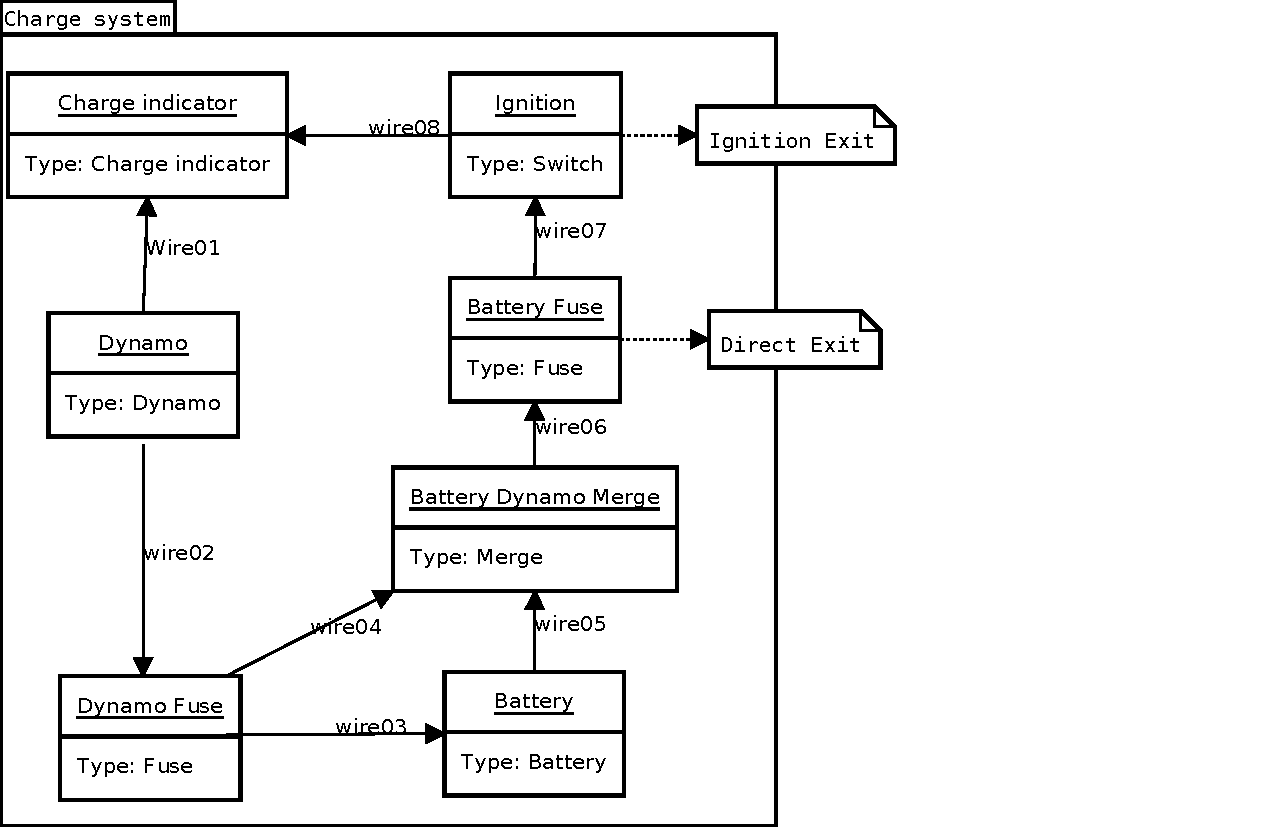
\includegraphics[width=1.00\textwidth]{ChargeSystem.pdf}
	\caption{The charge system of our example car}
	\label{fig:ChargeSystem}
\end{figure}

\begin{figure}[htbp]
	\centering
		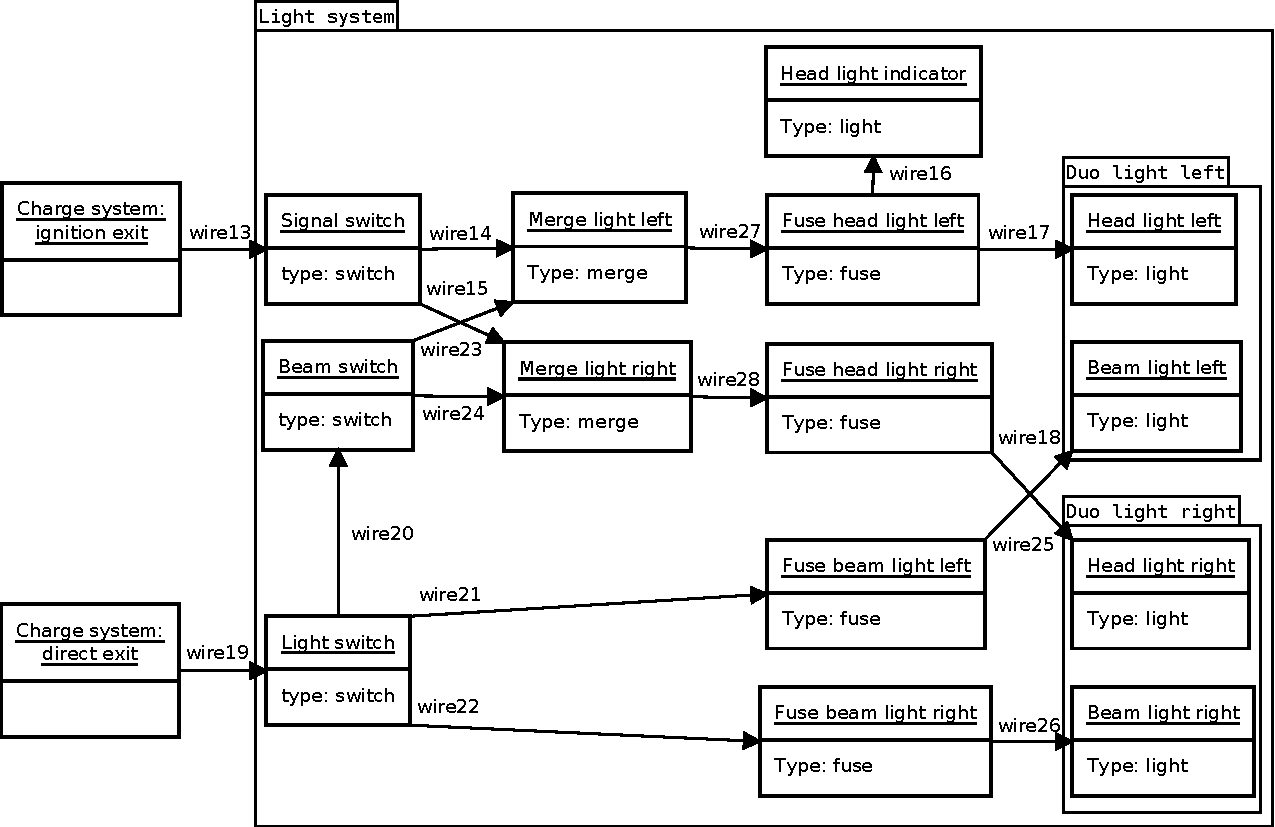
\includegraphics[width=1.00\textwidth]{LightSystem.pdf}
	\caption{The light system of our example car}
	\label{fig:LightSystem}
\end{figure}

\begin{figure}[htbp]
	\centering
		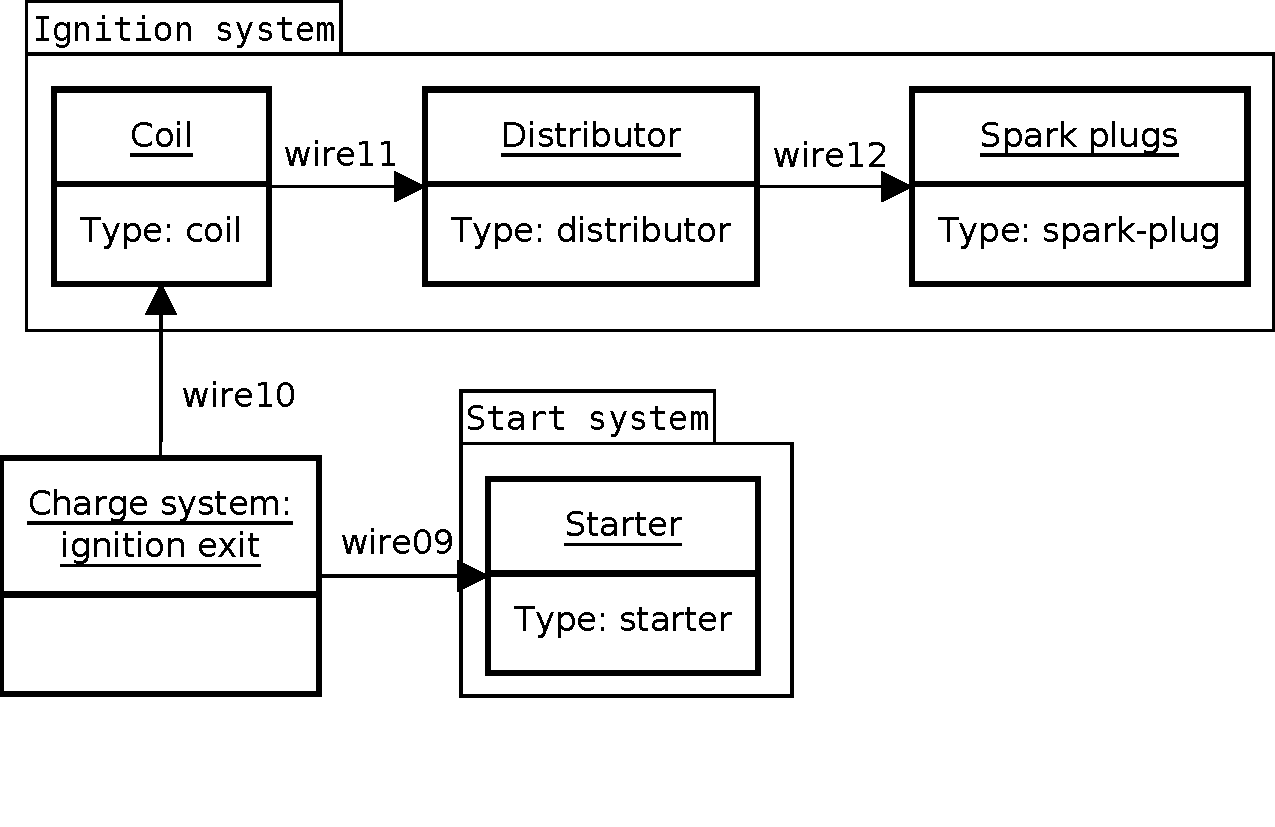
\includegraphics[width=1.00\textwidth]{StartAndIgnitionSystem.pdf}
	\caption{The start and the ignition system of our example car}
	\label{fig:StartAndIgnitionSystem}
\end{figure}


\subsection{Inference knowledge}
The inference model is shown in figure~\ref{fig:InferenceModel}. This inference
model is almost the same as the template shown in the CommonKADS book.
The first difference is an additional interaction with the user `obtain possible
selection'. This interaction was added because our user would greatly like to
influence the reasoning process by proposing his own hypothesis. The second
difference is the added transfer function `try to repair'. This is added because
the user has to try to repair his car to finally confirm an hypothesis. The model is
annotated with a simple example of how the system could work.

\begin{figure}[htbp]
	\centering
		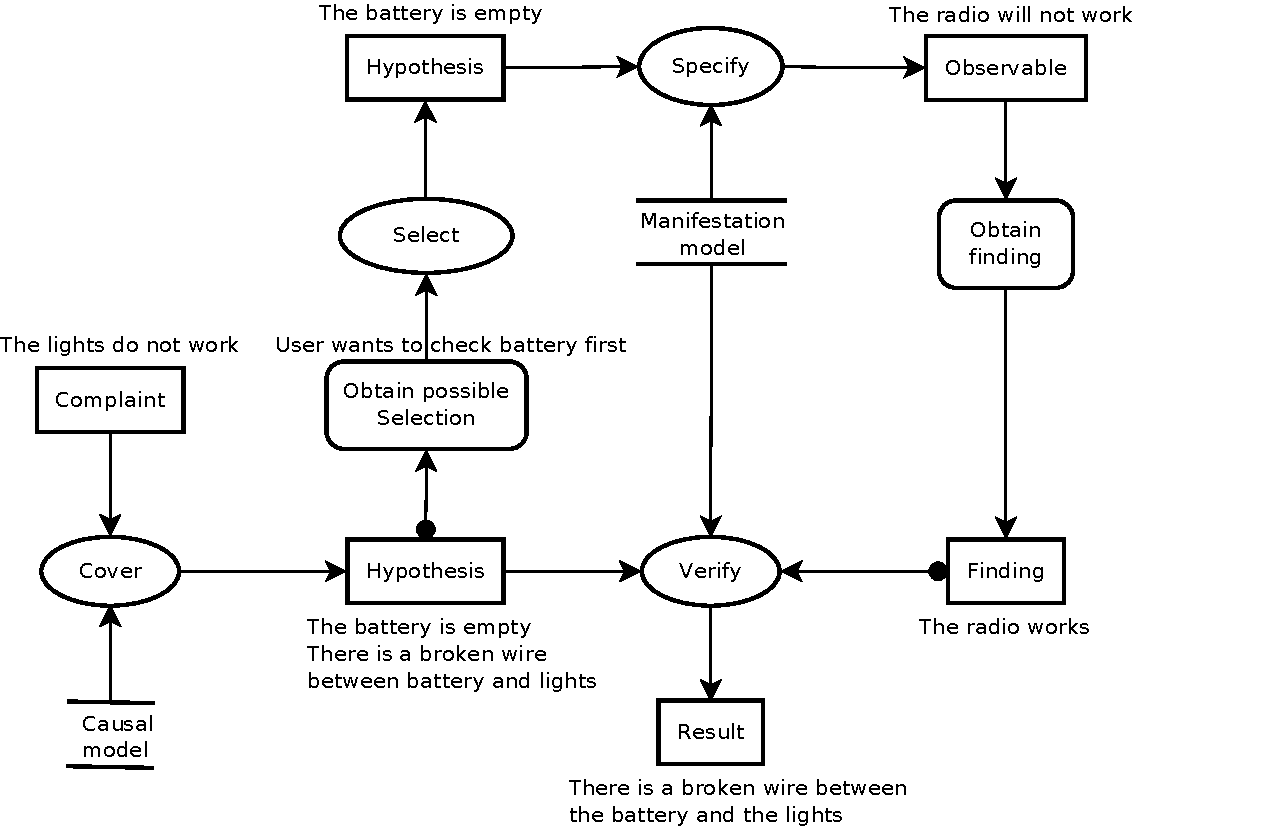
\includegraphics[width=1.00\textwidth]{inferenceModel.pdf}
	\caption{Annotated inference model}
	\label{fig:InferenceModel}
\end{figure}


\subsection{Task knowledge}
In our context analysis we identified to major task shown in the TM-1 tables.
For this project we decided to focus only on the diagnoses task. The task model
of the diagnoses task is shown in figure~\ref{fig:taskDecomposition}. The task
model shows that the diagnoses task consists of the inference and
interactions of the template diagnoses task plus the `obtain possible selection'
and `try to repair' transfer functions. `Obtain possible selection' is used for 
improved user interaction about hypothesis.
`Try to repair' is used to to ask the user to repair the car and confirm or
reject an hypothesis.

The task method we use to solve this task is in figure~\ref{fig:taskMethod}.
\begin{verbatim}
TASK diagnosis
  ROLES:
    INPUT:
      complaint: "Finding that initiates the diagnostic process";
    OUTPUT:
      faults: "The faults that could have caused the complaint";
      evidence: "The evidence gathered during diagnosis";
END TASK diagnosis;

TASK-METHOD augmented-causal-covering
  REALIZES: diagnosis
  DECOMPOSITION:
    INFERENCES: cover, select, specify, verify;
    TRANSFER-FUNCTIONS: obtain-possible-selection, obtain-finding,
        try-to-repair;
  ROLES:
    INTERMEDIATE:
      differential: "candidate solutions";
      hypothesis: "candidate solution";
      observable: "something that can be observed";
      finding: "the resulting information of an observation";
      repair-succesfull: "boolean indication result of the repair";
  CONTROL-STRUCTURE:
    cover(complaint -> differential);
    REPEAT WHILE differential.size == 0
      select(differential -> hypothesis);
      obtain-possible-selection(differential + hypothesis -> hypothesis);
      specify(hypothesis -> observable);
      IF "observables left" THEN
        obtain(observable -> finding);
        evidence := finding ADD evidence;
        verify(evidence + differential -> differential);
      ELSE
        try-to-repair(hypothesis -> repair-succesfull);
        IF NOT repair-succesfull THEN
          differential SUBSTRACT hypothesis;
        END IF
      END IF
    UNTIL repair-succesfull
    faults := differential;
END TASK-METHOD

\end{verbatim}
\begin{figure}[htbp]
	\centering
	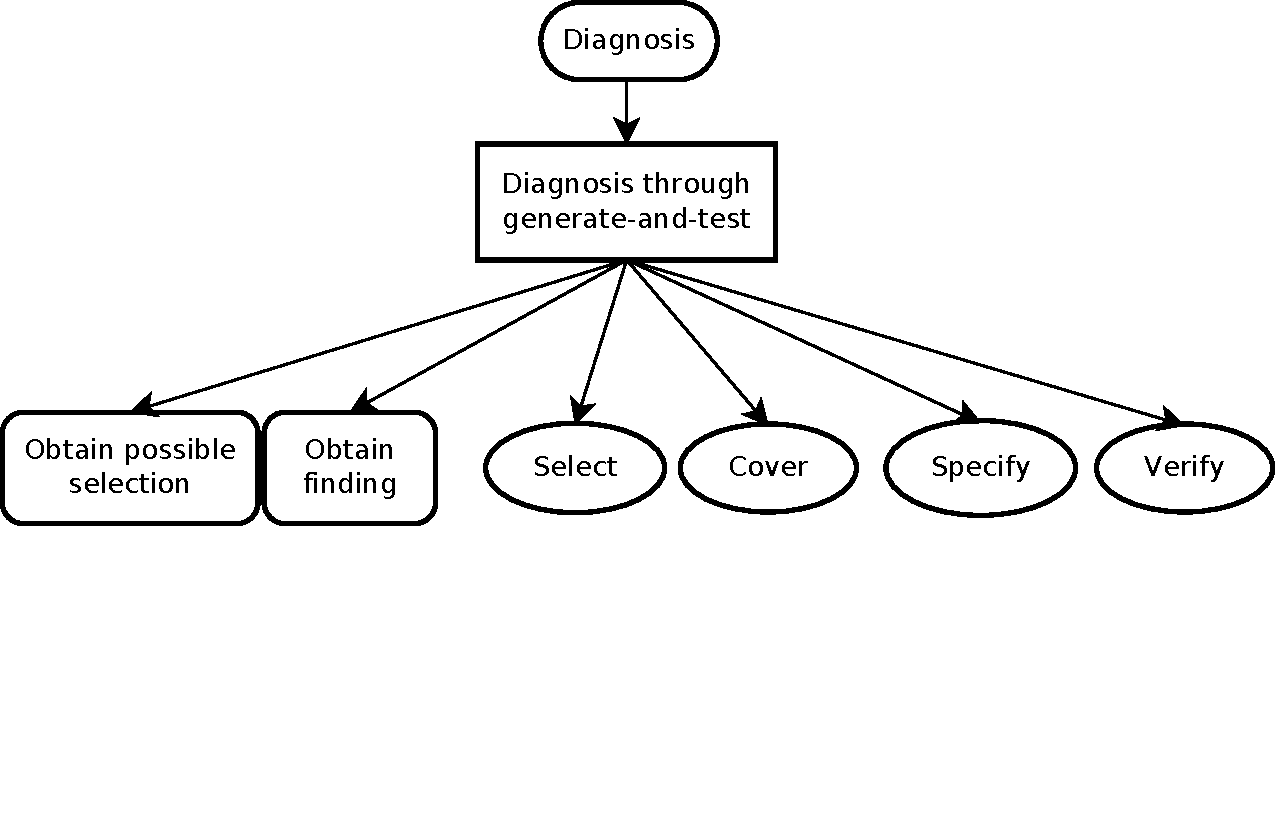
\includegraphics[width=1.00\textwidth]{taskDecomposition.pdf}
	\caption{Task-decomposistion diagram for the diagnoses task}
	\label{fig:taskDecomposition}
\end{figure}


\begin{figure}[htbp]
    \centering
    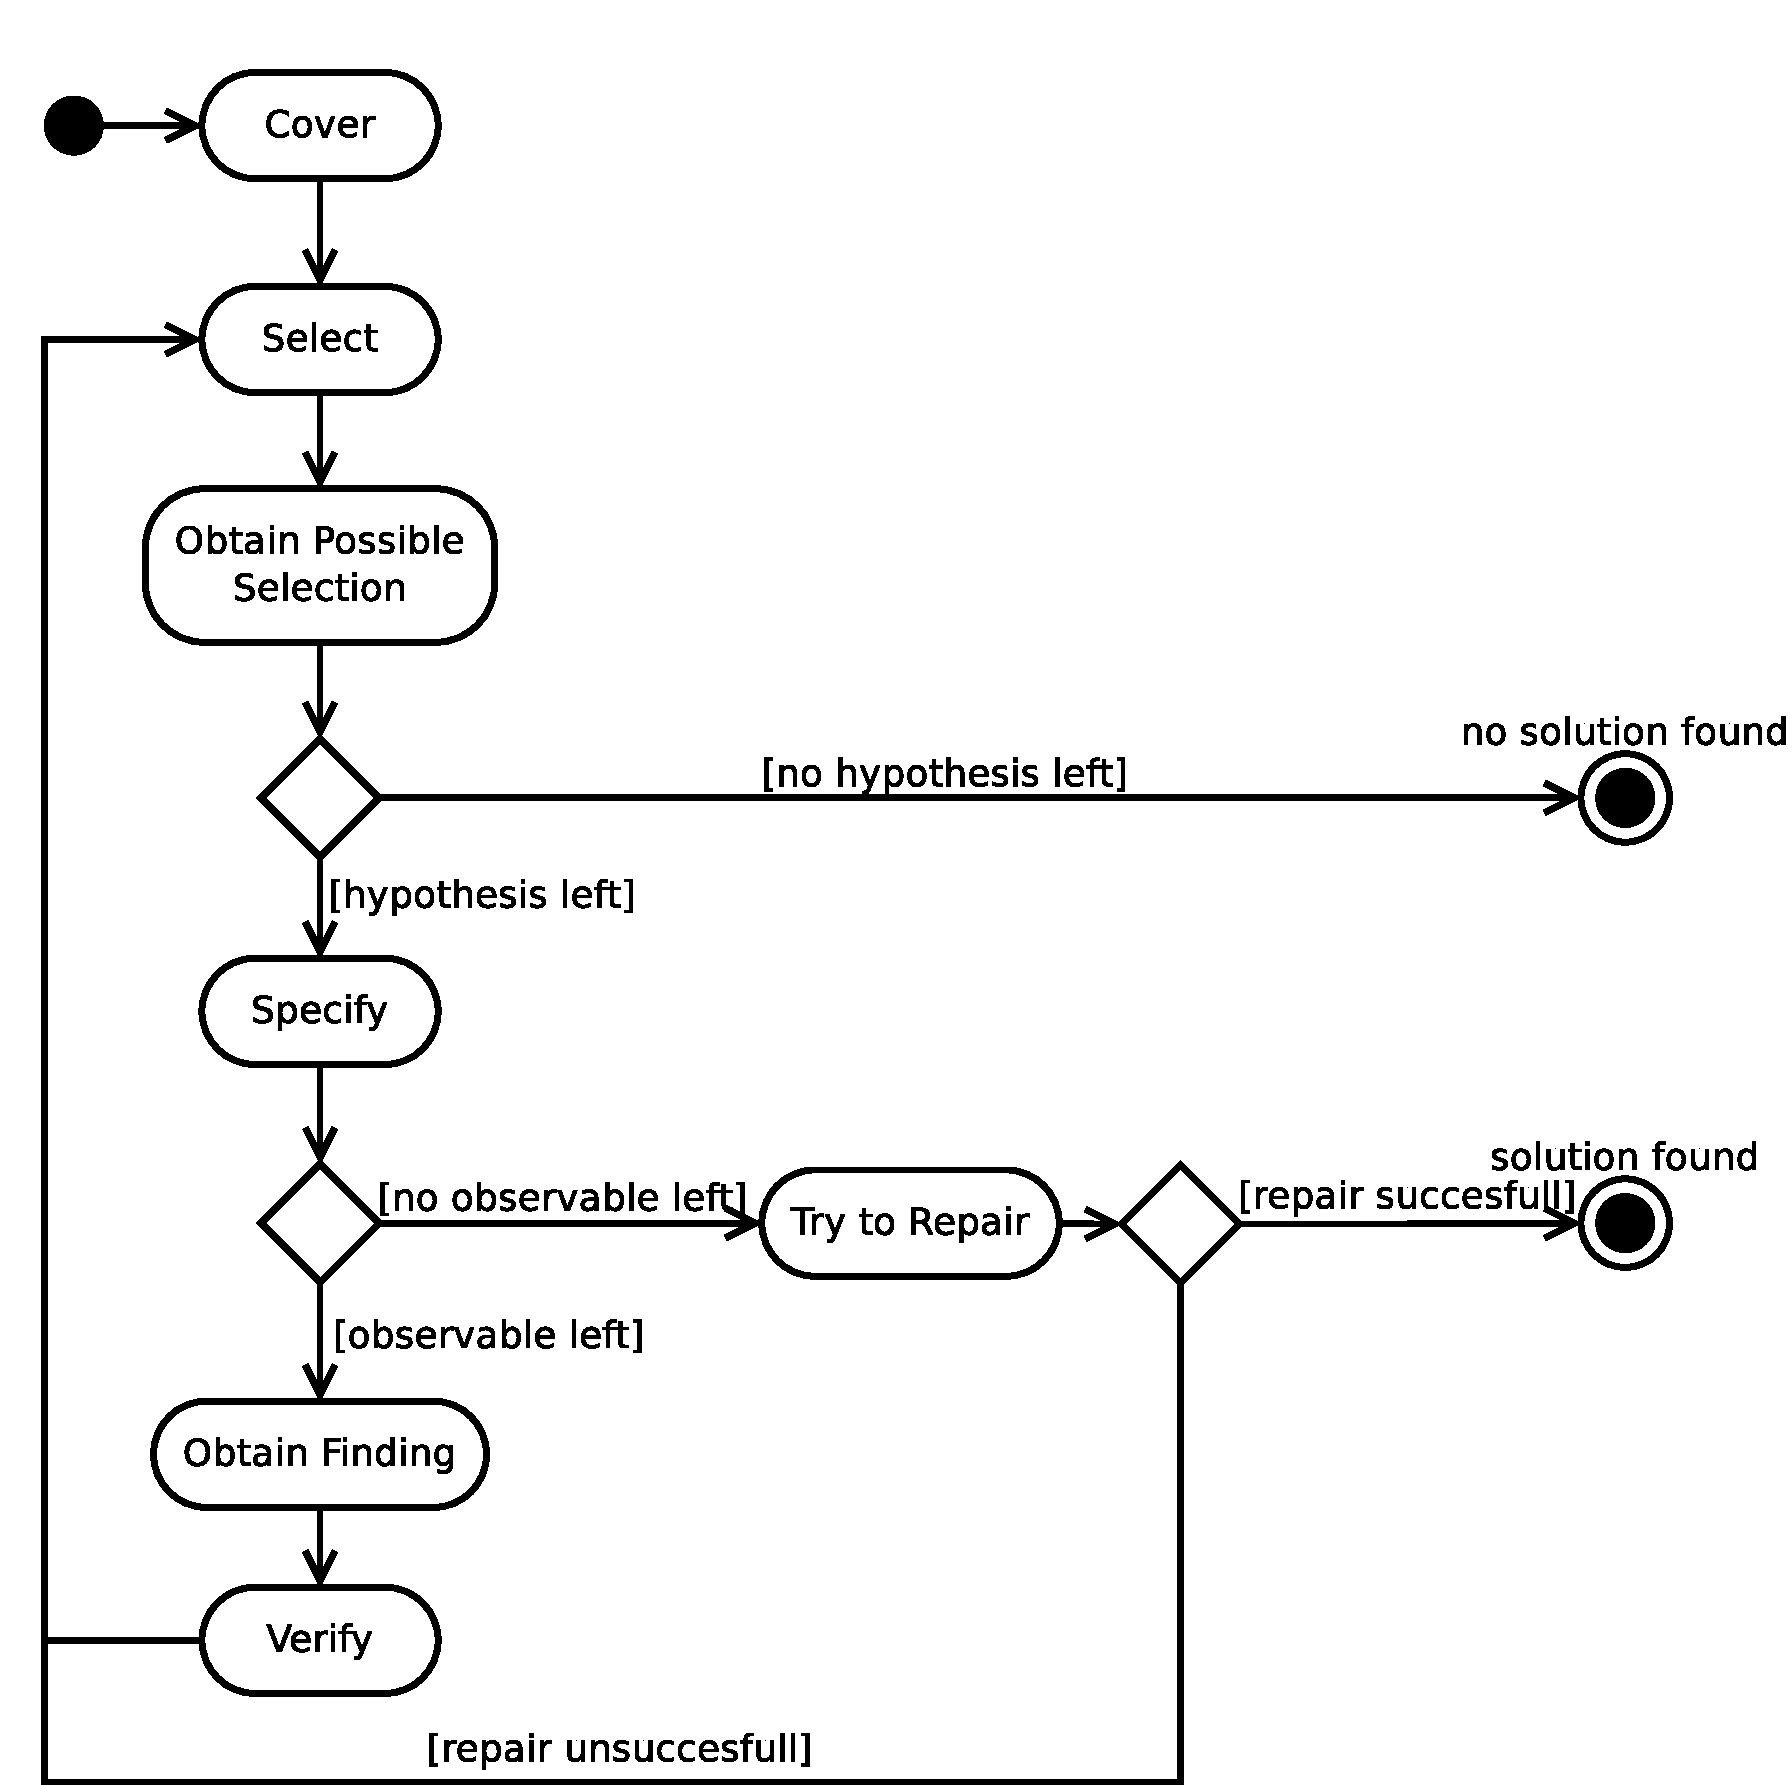
\includegraphics[width=1.00\textwidth]{task-method.pdf}
    \caption{The task method for our diagnosis task.}
    \label{fig:taskMethod}
\end{figure}
